\documentclass{article}
\usepackage{graphicx} % Required for inserting images
\usepackage[utf8]{inputenc}
\usepackage[russian]{babel}
\usepackage{enumitem}
\usepackage[T2A]{fontenc}
\usepackage{tocloft}
\usepackage{hyperref} 
\usepackage{tikz}
\usepackage{graphicx}

\renewcommand{\contentsname}{}

\title{Дизайн документ\\  «Escape the Matrix»}
\author{\\Куракина Юлия Вячеславовна}
\date{Ноябрь 2024}

\begin{document}

\maketitle

\tableofcontents 

\newpage
\section{Введение}

Данный документ описывает игру \textbf{«Escape the Matrix»}.\\ \\Содержание документа приведено на 1-2 страницах. \\Данный документ не является документом в форматах «EULA» или «Terms Of Use», он также не является коммерческой тайной. \\Документ написан на основании информации в общем доступе, полученной с веб-сервиса «GitHub»: \url{https://github.com/JuliaK434/Escape-the-Matrix} \\Документ менялся в период с ноября 2024 по апрель 2025 года.
\\Команда гейм-дизайнеров документа: Куракина Юлия Вячеславовна.\\Разработчики игры \textbf{«Escape the Matrix»}: Куракина Юлия Вячеславовна, Сергеев Максим Викторович, Дрямин Даниил Александрович. \\Сокращения и определения используются на основании документа \textbf{"Стандарт ГОСТ Р 53114-2008 «Защита информации. Обеспечение информационной безопасности в организации. Основные термины и определения»"}, других равносильных документов, также в документе могут использоваться общепринятые в обществе сокращения и определения. \\Дополнительных сведений для прочтения дизайн документа \textbf{не требуется}.

\newpage

\section{Концепция}

\paragraph{\textbf{Почему стоит обратить внимание на дизайн-документ:}}
Данный дизайн-документ является единственным в своём роде описанием игры «Escape the Matrix». Пользователь может ознакомиться с уникальностью данного проекта и протестировать продукт по вышеуказанной ссылке на «GitHub». Рекомендуется к прочтению тем, кто хочет ознакомиться с лором игры, её детальным функционалом и этапами разработки.
\paragraph{\textbf{Сюжет:}}
\textit{Главный герой игры — программист по имени Нуль, который неожиданно осознает, что живет внутри симуляции (Матрицы). Чтобы обрести свободу, ему нужно решить серию головоломок, каждая из которых приближает его к выходу из системы. По мере прохождения игрок узнает фрагменты истории персонажа и раскрывает тайны Матрицы.
}

\subsection{Введение}

\paragraph{\textbf{Суть игры:}}
"Escape the Matrix" — это головоломка с элементами квеста, где игрок должен анализировать окружение, находить скрытые подсказки и решать логические задачи, чтобы выбраться из виртуального мира. Игра сочетает атмосферу киберпанка и одноименного фильма "Матрица".

\subsection{Жанр и аудитория}
\begin{itemize}
\item 2D-головоломка, квест с элементами пазла.
\item Изометрическая игра – камера смотрит строго сверху, практически не меняя своего ракурса.
\end{itemize}

\subparagraph{Сеттинг:} Виртуальный мир, полный загадок.
\subparagraph{Целевая аудитория:} 12+ 
\begin{itemize}
\item Любящие интеллектуальные испытания.
\item Поклонники антиутопий, киберпанка и научной фантастики.
\item Те, кто ценит нарратив через геймплей, а не через длинные кат-сцены.
\end{itemize}
\subsection{Основные особенности игры}
USP – unique sellingpoints или ключевые особенности игры заключаются в ярком, неоновом, местами темном и фантастическим дизайне уровней. Простота и ясность "геймплея" добавляют особую атмосферу в прохождении, а нарастание сложности вызывает любопытство и интерес к финалу игры.
Также игра очень разнообразна на головоломки, что позволит любому игроку прокачать логику. 

\subparagraph{Обьём игры расчитан на ~ 30 минут}

\subsection{Описание игры}
Игрок перемещается по различным локациям, где стены, платформы и объекты подчиняются "правилам системы". Чтобы продвинуться, нужно:
\begin{enumerate}
\itemНаходить скрытые символы и коды.
\itemУметь расшифровывать шифры.
\itemЛогически рассуждать.
\itemВзаимодействовать с ошибками в матрице (глитчи, аномалии).
\end{enumerate}
Финал игры — выход из симуляции, но финал предлагает 2 варианта событий: выйти из матрицы или остаться в ней.
\paragraph{Элементы управления:}
Движение вправо/влево: кнопками "A" и "D" соответственно.\\
Движение вверх/вниз: кнопками "W" и "S" соответственно.
  Прыжок: клавиша пробел.\\
    Пауза: кнопка "пауза" на экране.\\
      Главное меню: кнопки "Значок Play»", "Значок Настройки", "Значок Выход из игры".

\subparagraph{Задача игрока:} Дойти до конца, постепенно решая головоломки.

\subsection{Предпосылки создания}
Проект разрабатывается как демонстрация навыков геймдизайна и работы с движком Unity. Вдохновившись фильмом "Матрица", а так же такими играми как:  "Portal", "The Talos Principle", "Antichamber", нашей команде захотелось создать компактную, но насыщенную головоломку, где каждая механика работает на атмосферу и сюжет.

\subsection{Платформа}

\begin{center}
    \begin{tabular}{|p{4cm}|p{4cm}|p{6cm}|}
    \hline
      \textit{\textbf {Требования}}   & \textit{\textbf {Минимальные}}  & \textit{\textbf {Рекомендуемые}}  \\
      [0.5ex]
      \hline 
        \textit{\textbf {Операционная система}} & ОС Windows 7 (64-bit) & ОС Windows 11 (64-bit)\\
        \hline 
         \textit{\textbf {Процессор}} & Intel Core 2 Duo & Intel Core i3 или лучше\\
         \hline
         \textit{\textbf {ОЗУ}} & 2 ГБ & 4 ГБ\\
         \hline
         \textit{\textbf {Свободное место на HDD}} & 1 ГБ& 2 ГБ\\
         \hline
         \textit{\textbf {Видео карта}} & Встроенная видеокарта с поддержкой DirectX 9 & видеокарта с поддержкой DirectX 11 или выше\\
         \hline
         \textit{\textbf {Звуковая карта}} & Любая совместимая с Windiws & Любая совместимая с Windiws\\
         \hline
         \textit{\textbf {Управление}} & Клавиатура и мышь/трекпад & Клавиатура и мышь/трекпад\\ 
         \hline  
         \textit{\textbf {Unity}} & Версия Unity 6 (6000.0.23f1) &Версия Unity 6 (6000.0.23f1)\\ [1ex]
         \hline  
    \end{tabular}
\end{center}

\newpage
\section{Функциональная спецификация}

\subsection{Принципы игры}

\subsubsection{Суть игрового процесса}
Игровой процесс в \textit{Escape the Matrix} строится на трёх ключевых элементах:

\begin{itemize}
    \item \textbf{Исследование локаций}:
    \begin{itemize}
        \item Игрок изучает постепенно искажающийся дом, обнаруживая аномалии и интерактивные объекты
        \item Каждый уровень добавляет новые визуальные изменения и механические сложности
    \end{itemize}
    
    \item \textbf{Решение головоломок}:
    \begin{itemize}
        \item Разнообразные типы задач: шифры (числовой, Цезаря, клавиатурный), пазл, лабиринт
        \item Головоломки требуют логического мышления и внимания к деталям окружения
    \end{itemize}
    
    \item \textbf{Взаимодействие с системой}:
    \begin{itemize}
        \item Управление персонажем через WASD
        \item Использование клавиши E для взаимодействия с объектами
        \item Меню паузы с возможностью настройки звука
    \end{itemize}
\end{itemize}

\subsubsection{Ход игры и сюжет}
Игра представляет собой нарративную головоломку с последовательным развитием:

\begin{enumerate}
    \item \textbf{Начало}:
    \begin{itemize}
        \item Персонаж оказывается в обычном доме (уровень 1)
        \item Первые простые взаимодействия знакомят с механиками
    \end{itemize}
    
    \item \textbf{Развитие}:
    \begin{itemize}
        \item Постепенное появление аномалий (уровни 2-3)
        \item Усложнение головоломок и увеличение интерактивных объектов
        \item Монологи персонажа раскрывают его восприятие изменяющейся реальности
    \end{itemize}
    
    \item \textbf{Кульминация}:
    \begin{itemize}
        \item Максимальные искажения на уровне 3 (хаотичные текстуры, плавающие объекты)
        \item Самые сложные комбинированные головоломки
        \item Исследование локации "офис" и решение головоломок.
    \end{itemize}
    
    \item \textbf{Развязка}:
    \begin{itemize}
        \item Возврат к стабильности на уровне 5
        \item Открытие меню выбора уровней как финальная награда
    \end{itemize}
\end{enumerate}

Сюжет подаётся через:
\begin{itemize}
    \item Визуальные изменения окружения
    \item Монологи персонажа с эффектом печатающегося текста
    \item Прогрессию сложности головоломок
    \item Контраст между "нормальным" и искажённым состояниями дома
\end{itemize}

\subsection{Персонаж игрока}
Нуль (Null) – минималистично и идеально для цифрового мира.
\begin{figure}[h] 
    \centering 
    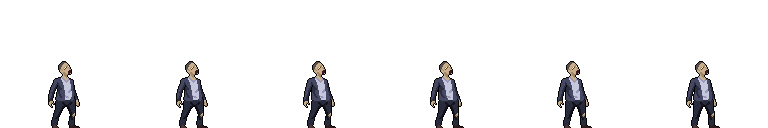
\includegraphics[width=0.8\textwidth]{Idle.png}
    \caption{Главный герой (состояние покоя)} \
    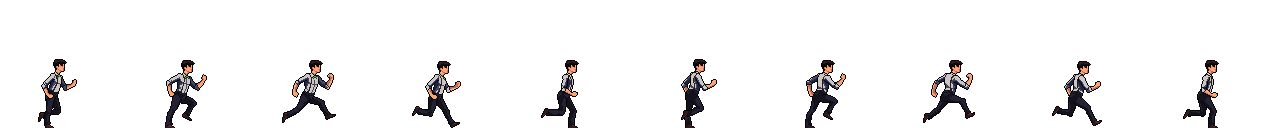
\includegraphics[width=0.8\textwidth]{Run.png}
    \caption{Главный герой (состояние бега)} \
\end{figure}

\subsection{Элементы игры}
Основные игровые элементы можно классифицировать следующим образом:

\begin{table}[h]
\centering
\begin{tabular}{|l|l|l|}
\hline
\textbf{Тип элемента} & \textbf{Примеры} & \textbf{Назначение} \\ \hline
Персонажи & Главный герой & Аватар игрока в мире игры \\ \hline
Объекты окружения & Двери, мебель & Создание игрового пространства \\ \hline
Интерактивные объекты & Компьютер, холодильник & Механики взаимодействия \\ \hline
Головоломки & Шифры, пазлы & Игровые вызовы \\ \hline
Декорации & Аномалии & Атмосфера и визуальный стиль \\ \hline
\end{tabular}
\caption{Классификация игровых элементов}
\label{tab:game_elements}
\end{table}

\subsection{Интерфейс пользователя}

\subsubsection{Функциональное описание и управление}
\begin{table}[h]
\centering
\begin{tabular}{|l|l|l|}
\hline
\textbf{Элемент} & \textbf{Управление} & \textbf{Функция} \\ \hline
Главное меню & Мышь & Навигация по пунктам (играть, настройки, выход из игры) \\ \hline
Меню паузы & Мышь & Управление игровым процессом (Продолжить, выйти из игры) \\ \hline
Диалоги & Пробел/мышь & Продвижение по сюжету \\ \hline
\end{tabular}
\caption{Функциональные элементы управления}
\label{tab:ui_controls}
\end{table}

\subsubsection{Объекты интерфейса пользователя}
Основные UI-компоненты реализованы в Unity Canvas:

\begin{itemize}
\item \textbf{Кнопки}:
\begin{itemize}
\item Стандартный размер: 200x50 пикселей
\item Эффект нажатия
\end{itemize}

\item \textbf{Текстовые поля}:
\begin{itemize}
\item Шрифт: PixeloidSans 
\item Эффект Typewriter для диалогов
\end{itemize}

\item \textbf{Ползунки}:
\begin{itemize}
\item Громкость: диапазон 0-100\%
\end{itemize}

\item \textbf{Панели}:
\begin{itemize}
\item Прозрачность: 85\%
\item Округление углов
\end{itemize}
\end{itemize}

\begin{figure}[h]
\centering
\includegraphics[width=0.7\textwidth]{UI.jpg}
\caption{Визуальные компоненты UI}
\label{fig:ui_components}
\end{figure}

\subsection{Графика и видео}

\subsubsection{Общее описание}
Графический стиль игры сочетает пиксель-арт эстетику с элементами киберпанка. Основные характеристики:

\begin{itemize}
    \item \textbf{Разрешение}: 1920x1080 (Full HD) с поддержкой 1280x720
    \item \textbf{Цветовая палитра}: Доминирующие зелёные и чёрные тона, яркие неоновые для киберпанк локаций.
    \item \textbf{Инструменты}: Photoshop/Pixilart, itch.io/AssetStore  (спрайты), Unity Animator (анимации).
\end{itemize}
\subsubsection{Двумерная графика и анимация}
Основные графические элементы реализованы через систему спрайтов:

\begin{table}[h]
    \centering
    \begin{tabular}{|l|c|c|}
        \hline
        \textbf{Элемент} & \textbf{Размер (px)} & \textbf{FPS} \\ \hline
        Персонаж & 64x64 & 12 \\ \hline
        Объекты локаций & 32x32 - 128x128 & 8 \\ \hline
        Эффекты аномалий & 256x256 & 24 \\ \hline
    \end{tabular}
    \caption{Параметры графических элементов}
    \label{tab:gfx}
\end{table}

\subsubsection{Музыка}
Музыка взята из открытых источников с разрешением на коммерческое использование. Жанр - \textbf{электронная}. На протяжении всей игры играют 3 трека. 

\subsection{Описание уровней}
\begin{enumerate}[label=\arabic*., leftmargin=*]
    \item \textbf{1 уровень}\\
    \textbf{Начало}\\
    ГГ просыпается у себя в спальне и решает шифр.
\item \textbf{2-3 уровень}\\
Повторяется принцип и локации 1-го уровня. С каждым уровнем сложность квестов повышается и добавляются новые головоломки. 
\item \textbf{4 уровень}\\
\\ \textbf{Оффис}\\
 ГГ тестируют на агента матрицы. Игрок выполняет квесты.
 \item \textbf{5 уровень}\\
 \\ \textbf{Осознание}\\
 ГГ просыпается в своем доме, к нему подходит персонаж из фильма "Матрица" и рассказывает всю правду, Задаёт вопрос кто ты? Игроку даётся возможность походить по локации игры. Правильный ответ: \textbf{Личность} Финал имеющий 2 концовки, философский вопрос игроку: "Свободен ли ты?"
        \begin{itemize}
            \item Ответ "Да" - открывает выбор уровней
            \item Ответ "Нет" - статичный финальный экран
        \end{itemize}
\end{enumerate}

\subsubsection{Общее описание дизайна уровней}
\subsection*{1. Концепция и структура уровней}
Уровни в игре \textit{Escape the Matrix} спроектированы с учётом принципов постепенного усложнения и нарративной целостности. Первые три уровня и пятый уровень представляют собой локацию \textit{«Дом»}, которая визуально и механически трансформируется по мере прогресса игрока. На 4 уровне игрока ожидает локация офиса в стиле киберпанк. Основные особенности:
\begin{itemize}
    \item \textbf{Прогрессия аномалий}: 
    \begin{itemize}
        \item \textit{Уровень 1}: Отсутствие аномалий, «нормальное» состояние дома.
        \item \textit{Уровень 2}: Появление первых искажений (изменение цветов объектов, включение электроники).
        \item \textit{Уровень 3}: Максимальные искажения (хаотичные текстуры, «плывущие» окна, добавление новых объектов).
        \item \textit{Уровень 5}: Возврат к стабильности (финальная локация без аномалий).
    \end{itemize}
    \item \textbf{Стилистика}: Пиксель-арт с преобладанием зелёной цветовой гаммы (отсылка к «Матрице»). Камера — фиксированный вид сверху (top-down 2D).
\end{itemize}

\subsection*{2. Ключевые игровые механики на уровнях}
\begin{table}[h]
    \centering
    \begin{tabular}{|l|l|l|}
        \hline
        \textbf{Уровень} & \textbf{Головоломки} & \textbf{Интерактивные объекты} \\ \hline
        1 & Числовой шифр & Шкаф, дверь \\ \hline
        2 & Шифр Цезаря, пазл & Компьютер, кресло \\ \hline
        3 & Лабиринт, клавиатурный шифр & Холодильник, собака, телефон \\ \hline
        4 & Логическая цепочка действий для достижения цели &  -\\ \hline
        5 & Диалог с боссом & Дверь для перехода в меню \\ \hline
    \end{tabular}
    \caption{Распределение механик по уровням}
\end{table}

\subsection*{3. Техническая реализация}
\begin{itemize}
    \item \textbf{Локации}: 
    \begin{itemize}
        \item Созданы на основе атласов спрайтов (нарезка в \textit{Unity Sprite Editor}).
        \item Коллизии настроены через \textit{CapsuleCollider2D} (для плавного взаимодействия).
        \item Аномалии реализованы заменой спрайтов через события (напр., после решения головоломки).
    \end{itemize}
    \item \textbf{Навигация}: 
    \begin{itemize}
        \item (1, 2, 3, 5 уровни) Фиксированная камера, (4 уровень) камера следует за игроком.
        \item Переходы между сценами через \textit{SceneManager.LoadScene()}.
    \end{itemize}
\end{itemize}

\subsection*{4. Баланс и тестирование}
Уровни тестировались на 10 пользователях. Ключевые метрики:
\begin{itemize}
    \item Среднее время прохождения уровня: 3--5 минут.
    \item Коэффициент успешности головоломок: 90--100\%.
\end{itemize}
Корректировки после тестов:
\begin{itemize}
    \item Уменьшение фрагментов пазла с 25 до 6 (для снижения времени решения).
    \item Добавление звёзд в лабиринт (увеличение сложности).
\end{itemize}

\subsection*{5. Перспективы доработки}
\begin{itemize}
    \item Добавление procedural generation для вариативности локаций.
    \item Введение динамической камеры для крупных планов на ключевые объекты.
    \item Расширение системы аномалий (например, случайные события).
\end{itemize}

\newpage

\section{Контакты}

\textbf{Куракина Юлия Вячеславовна} - Дизайн и программирование пользовательского интерфейса (UI/UX), игровые механики (ivkurakina@edu.hse.ru)\\
\textbf{Курятников Дмитрий Максимович} - Программирование искусственного интеллекта для NPC, игровые механики (dmkuriatnikov@edu.hse.ru)\\
\textbf{Сергеев Максим Викторович} - Реализация системы достижений и наград (mvsergeev@edu.hse.ru)\\
\textbf{Дрямин Даниил Александрович} - Тестирование и отладка (dadriamin@edu.hse.ru)\\
\end{document}
